% !TEX root = ../main.tex
\begin{figure}[!p]
    \centering
    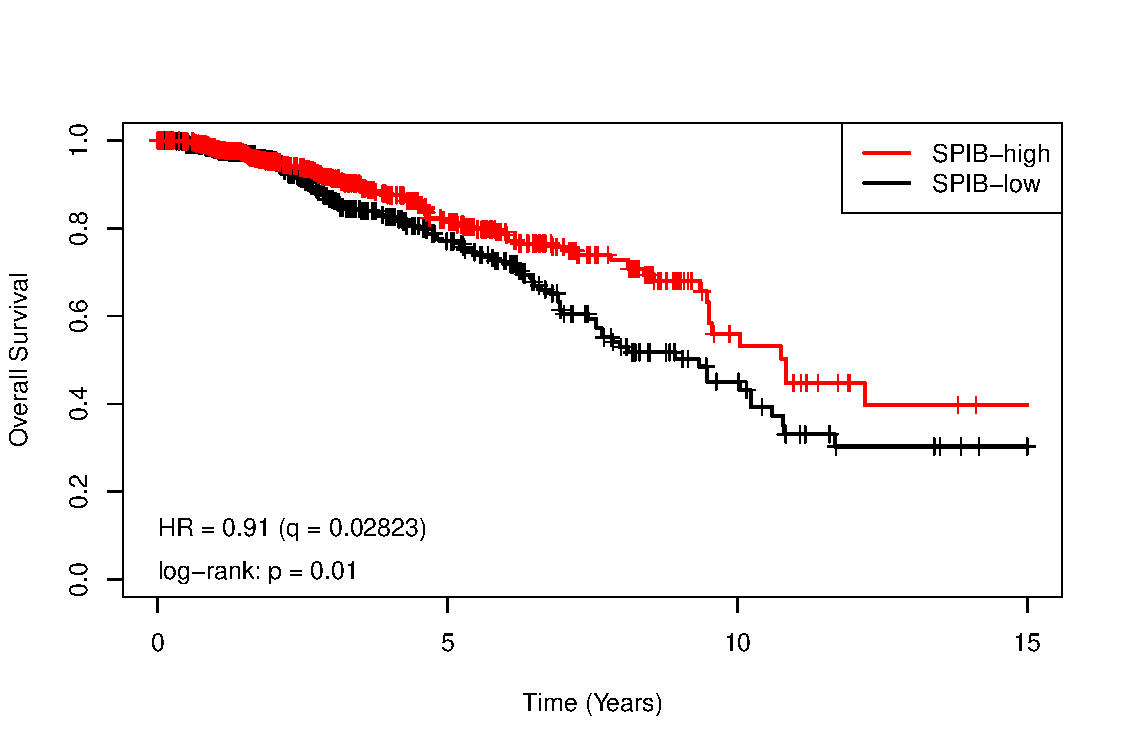
\includegraphics[scale=0.70]{figures/km_plot.pdf}
    \caption{Survival of SPIB-high and SPIB-low breast cancer patients. Data from the TCGA BRCA dataset \cite{Ciriello2015, Goldman2018}.}
    \label{km_plot}
\end{figure} 
\clearpage
\begin{table}[!p]
    \centering
    \caption{Methylation Sites}
    \begin{center}
    \begin{tabular}{l|lllll}
        CpG & cor & p-value & q-value & Mean (SPIB-High) & Mean (SPIB-Low) \\ \hline
        cg07979271 & $-0.514$ & $5.55 \cdot 10^{-60}$ & $9.43 \cdot 10^{-59}$ & $0.816$ & $0.864$\\ 
        cg13403724 & $0.288 $& $3.80 \cdot 10^{-18}$ & $3.23 \cdot 10^{-17}$ & $0.248$ & $0.206$\\ 
        cg17774764 & $-0.281$ & $3.07 \cdot 10^{-17}$ & $1.74 \cdot 10^{-16}$ & $0.737$ & $0.775$\\ 
        cg03763616 & $-0.277$ & $7.68 \cdot 10^{-17}$ & $3.26 \cdot 10^{-16}$ & $0.832$ & $0.859$\\ 
        cg19387862 & $0.272$& $2.70 \cdot 10^{-16}$ & $9.20 \cdot 10^{-16}$ & $0.191$ & $0.168$\\ 
        cg15690347 & $0.266$& $1.25 \cdot 10^{-15}$ & $3.54 \cdot 10^{-15}$ & $0.383$ & $0.301$\\ 
        cg08201854 & $0.265$& $1.87 \cdot 10^{-15}$ & $4.55 \cdot 10^{-15}$ & $0.26$ & $0.226$\\ 
        cg15007959 & $0.263$& $3.08 \cdot 10^{-15}$ & $6.55 \cdot 10^{-15}$ & $0.253$ & $0.203$\\ 
        cg18254819 & $0.246$& $1.53 \cdot 10^{-13}$ & $2.90 \cdot 10^{-13}$ & $0.235$ & $0.212$\\ 
        cg24092179 & $0.228$& $1.00 \cdot 10^{-11}$ & $1.71 \cdot 10^{-11}$ & $0.271$ & $0.244$\\ 
        cg22268231 & $-0.147$ & $1.22 \cdot 10^{-05}$ & $1.88 \cdot 10^{-05}$ & $0.45$ & $0.487$\\ 
        cg06512885 & $-0.133$ & $7.89 \cdot 10^{-05}$ & $0.000112$ & $0.875$ & $0.881$\\ 
        cg26522743 & $-0.0968$ & $0.0042$ & $0.00549$ & $0.394$ & $0.424$\\ 
        cg21152077 & $0.0921$ & $0.00653$ & $0.00792$ & $0.464$ & $0.448$\\ 
        cg13918544 & $0.0845$ & $0.0125$ & $0.0141$ & $0.132$ & $0.143$\\ 
        cg22745102 & $0.0705$ & $0.0372$ & $0.0396$ & $0.469$ & $0.462$\\ 
        cg04508467 & $2.02 \cdot 10^{-05}$ & $1$ & $1$ & $0.696$ & $0.686$\\ \hline
    \end{tabular}
    \end{center}
    Spearman correlation of methylation of CpG islands and the mRNA expression of SPIB.
    \label{meth_table}
\end{table} 
    
\clearpage
\begin{figure}[!p]
    \centering
    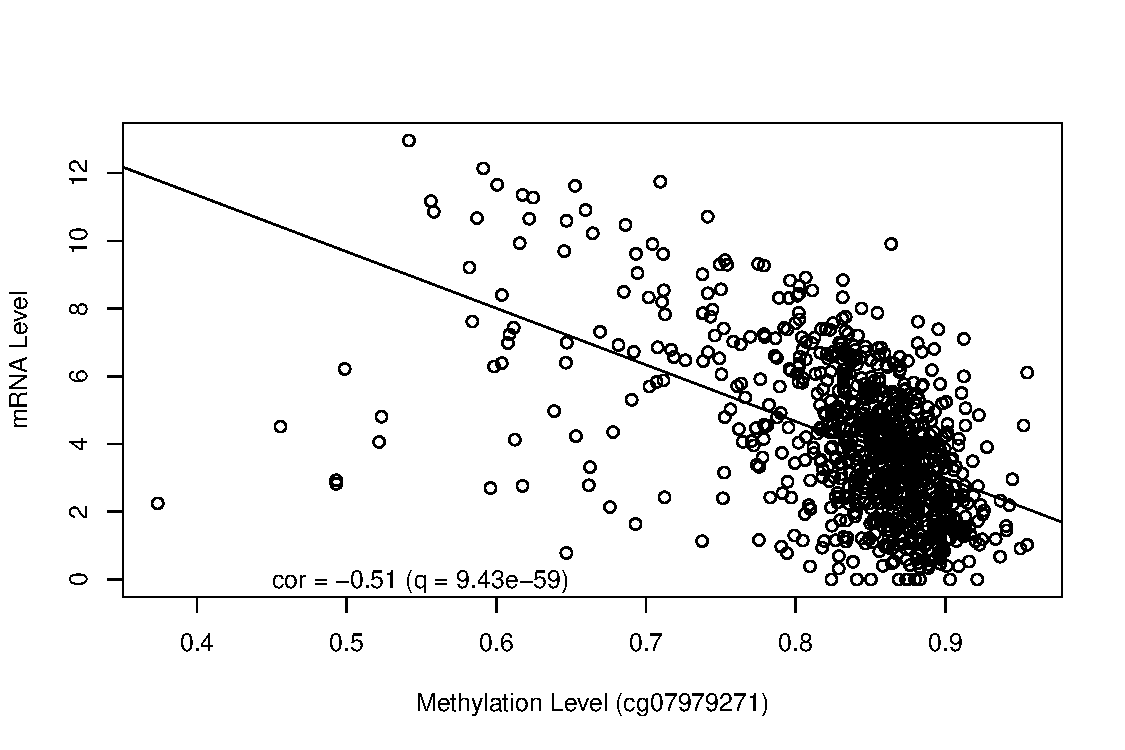
\includegraphics[scale=0.75]{figures/methylation.pdf}
    \caption{Scatter plot of SPIB methlyation vs mRNA expression values. Spearman correlation shown. Data from the TCGA BRCA dataset \cite{Ciriello2015, Goldman2018}.}
    \label{methylation}
\end{figure} 
\clearpage
\begin{figure}[!p]
    \centering
    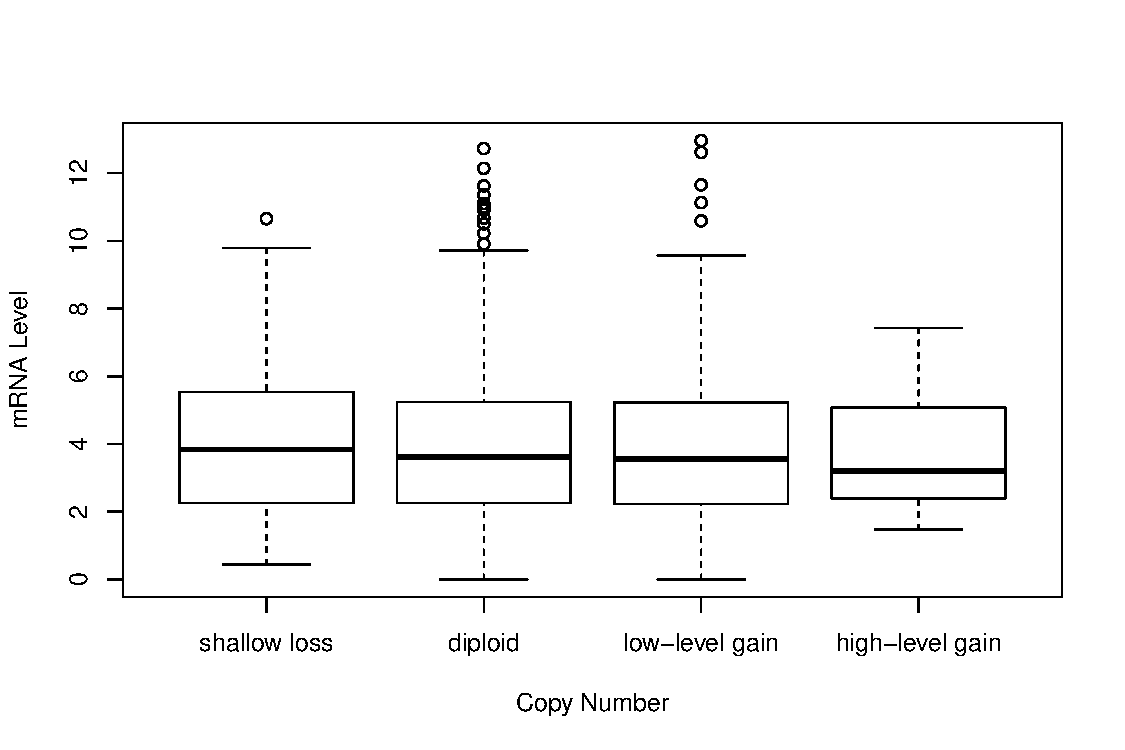
\includegraphics[scale=0.75]{figures/cnv.pdf}
    \caption{mRNA expression of SPIB compared under different copy number alteration levels. Data from the TCGA BRCA dataset \cite{Ciriello2015, Goldman2018}.}
    \label{cnv}
\end{figure} 
\clearpage
\begin{table}[!p]
    \centering
    \caption{mRNA Co-Expression}
    \begin{center}
    \begin{tabular}{l|lllll}
        Gene	&	Cor	&	p-value	&	q-value	&	Mean (SPIB-High)	&	Mean (SPIB-Low) \\ \hline
        MS4A1	&	0.822	&	2.95e-299	&	2.98e-295	&	6.88	&	3.16\\ 
        TCL1A	&	0.820	&	1.9e-296	&	1.28e-292	&	4.23	&	1.08\\ 
        CXCR5	&	0.819	&	3.59e-296	&	1.82e-292	&	5.15	&	2.59\\ 
        LCK	&	0.816	&	7.29e-292	&	2.95e-288	&	7.86	&	5.62\\ 
        ACAP1	&	0.811	&	1.52e-285	&	5.12e-282	&	7.44	&	5.15\\ 
        CCR7	&	0.809	&	5.04e-283	&	1.46e-279	&	7.26	&	4.9\\ 
        LTB	&	0.808	&	3.61e-282	&	9.13e-279	&	7.48	&	4.68\\ 
        CD5	&	0.801	&	4.46e-273	&	9.99e-270	&	7.41	&	5.13\\ 
        IL2RG	&	0.800	&	1.54e-272	&	3.13e-269	&	9.45	&	7.41\\ 
        CD6	&	0.799	&	9.15e-271	&	1.68e-267	&	7.86	&	5.84\\ 
        SIT1	&	0.795	&	4.51e-266	&	7.61e-263	&	5.92	&	3.67\\ 
        CD3D	&	0.795	&	5.73e-266	&	8.93e-263	&	7.12	&	4.79\\ 
        UBASH3A	&	0.792	&	5.48e-263	&	7.93e-260	&	5.31	&	3.02\\ 
        MAP4K1	&	0.792	&	1.64e-262	&	2.22e-259	&	7.39	&	5.55\\ 
        CD27	&	0.791	&	9.02e-262	&	1.14e-258	&	7.54	&	5.23\\ 
        SPOCK2	&	0.791	&	3.1e-261	&	3.69e-258	&	9.56	&	7.68\\ 
        CCL4	&	0.524	&	5.7e-87	&	2.66e-85	&	7.07	&	5.92\\ \hline
        DCTN4	&	-0.417	&	1.82e-52	&	4.77e-51	&	10.7	&	11.1\\ 
        FOXA1	&	-0.407	&	6.87e-50	&	1.7e-48	&	10.9	&	12\\ 
        PLA2G12A	&	-0.401	&	2.3e-48	&	5.47e-47	&	9.83	&	10.3\\ 
        FNIP1	&	-0.397	&	3.88e-47	&	9.03e-46	&	9.48	&	9.96\\ 
        USP30	&	-0.396	&	5.19e-47	&	1.21e-45	&	8.61	&	8.96\\ 
        GLRB	&	-0.393	&	2.47e-46	&	5.62e-45	&	6.61	&	7.61\\ 
        STRN3	&	-0.392	&	6.22e-46	&	1.4e-44	&	9.28	&	9.67\\ 
        TMEM192	&	-0.39	&	1.31e-45	&	2.92e-44	&	8.88	&	9.32\\ 
        RNF14	&	-0.384	&	3.89e-44	&	8.39e-43	&	10.3	&	10.6\\ 
    \end{tabular}
    \end{center}
    Spearman correlation of mRNA of multiple genes and the mRNA expression of SPIB. Upper half is sorted based on q-values (ascending). Lower half is sorted based on correlation coefficient (ascending).
    \label{mrna_table}
\end{table} 
    
\clearpage